% 第 1 章 分数次迭代问题
% 数值来源：仓库根目录 README.md 与 kneser 库（src/kneser）；第 2 章脚本 figures/ch02_sqrt2.py；
% 论文 [KneserPaper] 引言与 §3.1、§11。
\chapter{分数次迭代问题}\label{ch:intro}

给定一个映射 $f$，它的整数次迭代 $f^{\circ n}=f\circ\cdots\circ f$ 是明确的。
本书讨论的问题是：$f^{\circ 1/2}$、$f^{\circ t}$（$t$ 为实数）应当是什么。
这个问题在整数之外没有唯一答案。
本章先用两个具体例子（半指数函数和 tetration）说明问题，
再说明不唯一性从何而来、经典理论给出了哪两种答案，
最后陈述全书的中心论点和主定理，并给出各章的路线图。

本章的证明都很短。较长的经典证明放在第~\ref{ch:koenigs}~章及以后。

\begin{goals}
\item 分数次迭代由 \textbf{Abel 方程} $A\circ f=A+1$ 的一个解确定；Abel 方程的解相差一个 1-周期函数，因此分数次迭代不唯一（\cref{ch1:prop:nonunique}）。
\item 在实吸引不动点处，Koenigs 线性化给出一个自然的解，即\textbf{正则迭代}（regular iteration）。指数函数在实轴上没有不动点，Kneser 用一对复不动点构造了实解析的半指数函数。
\item 当映射有两个实不动点时，两个不动点各给出一个正则解。本书的中心论点是：\emph{分数次迭代是缝合两个不动点坐标的方式}，所有缝法之间的差别都记录在两个坐标的转移映射里。
\item 主定理（\cref{thm:main-preview}）描述两个不动点在鞍结中合并时转移映射的极限、展开与变分。
\end{goals}

% ------------------------------------------------------------------
\section{两个例子}\label{ch1:sec:examples}

\subsection{半指数函数}

是否存在实函数 $f:\R\to\R$ 使得
\begin{equation}\label{ch1:eq:halfexp}
  f(f(x))=\ee^{x}\qquad(x\in\R)?
\end{equation}
这样的 $f$ 称为\textbf{半指数函数}（half-exponential）。
先看几个初等事实。若 $f$ 连续且满足 \eqref{ch1:eq:halfexp}，则 $f$ 是单射（因为 $\exp$ 是单射），
所以严格单调；它不可能递减，否则 $f$ 有不动点 $x_0$，而 $\ee^{x_0}=f(f(x_0))=x_0$，
但 $\exp$ 在实轴上没有不动点（\cref{ch1:ex:increasing}）。
所以 $f$ 严格递增，并且 $f(x)>x$ 对一切 $x$ 成立。

\emph{连续}的解很容易构造，适当选取初始数据甚至可以得到 $C^\infty$ 的解。
例如任取 $c<0$ 和一个递增双射 $\varphi:(-\infty,c]\to(c,0]$，令 $f=\varphi$ 于 $(-\infty,c]$，
再用 $f(\varphi(x))=\ee^x$ 和 $f(\ee^x)=\ee^{f(x)}$ 依次把 $f$ 延拓到 $(c,0]$、$(0,\ee^c]$、$(\ee^c,1]$、……，就得到 $\R$ 上的一个连续递增解。
$\varphi$ 的选取是任意的，所以这种解有无穷多个。
真正的问题是：是否存在\emph{实解析}的解，是否有一个解比其他解更「自然」。

H.~Kneser 在 1950 年证明了实解析解的存在性~\cite{Kneser1950}。
他的构造（\cref{ch1:sec:kneser}）后来被 Trappmann 与 Kouznetsov 证明在一个复域条件下是唯一的~\cite{TrappmannKouznetsov2011}，
Paulsen 与 Cowgill 在另一组条件（在 $\C\setminus(-\infty,-2]$ 上全纯、实轴对称、在 $\pm\ii\infty$ 处的极限）下证明了 tetration 方程的唯一性~\cite{PaulsenCowgill2017}。
Kneser 的解没有闭式。仓库根目录的 \texttt{kneser} 库（\texttt{README.md}）用预先算好的 50 位系数计算它，例如
\begin{equation}\label{ch1:eq:halfexp-values}
\begin{aligned}
  f(0.5)&=1.0016400378866632\ldots, & f(f(0.5))&=1.648721270700128\ldots=\ee^{0.5},\\
  f(0)&=0.4985632879411144\ldots, & f(1)&=1.6463542337511945\ldots,
\end{aligned}
\end{equation}
并且 $f(x)\to-0.696024740886\ldots$（$x\to-\infty$）。
图~\ref{ch1:fig:halfexp} 画出了 $f$ 与 $\exp$。
这些数值取自仓库的 \texttt{README.md} 与 \texttt{docs/VALUES.md}（50 位表，此处截到双精度）；
其中 $f(0.5)$ 与 $f(f(0.5))$ 由脚本 \texttt{figures/fig1\_halfexp.py} 调用 \texttt{kneser} 库重新算出（数值）。

\begin{figure}[ht]
  \centering
  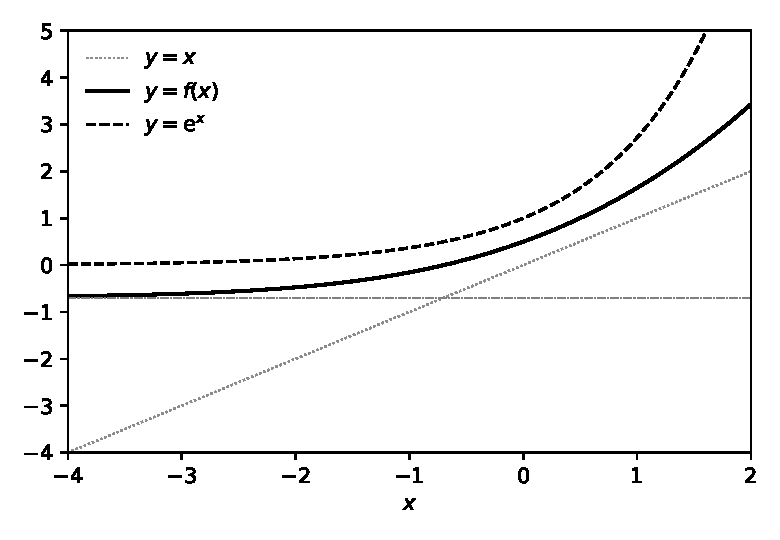
\includegraphics[width=0.62\textwidth]{figures/fig1_halfexp.pdf}
  \caption{Kneser 的半指数函数 $f$（实线）、$\ee^x$（虚线）与对角线。
  点划线是水平渐近线 $y=-0.69602\ldots$。脚本 \texttt{figures/fig1\_halfexp.py}。}
  \label{ch1:fig:halfexp}
\end{figure}

\subsection{Tetration}

与半指数函数等价的问题是解 \textbf{tetration 方程}（超指数方程）
\begin{equation}\label{ch1:eq:tetration}
  F(z+1)=b^{F(z)},\qquad F(0)=1 ,
\end{equation}
这里 $b>1$ 是底数。对正整数 $n$，$F(n)=b^{b^{\cdot^{\cdot^{b}}}}$（$n$ 个 $b$），
所以 $F$ 是把「$n$ 层指数塔」延拓到非整数高度的函数，记作 $\mathrm{sexp}_b$。
若 $\mathrm{sexp}_b$ 是 $\R$ 上（或 $(-2,\infty)$ 上）的严格递增函数，记它的反函数为 $\mathrm{slog}_b$，
则
\[
  f^{\circ t}(x):=\mathrm{sexp}_b\bigl(\mathrm{slog}_b(x)+t\bigr)
\]
满足 $f^{\circ 1}(x)=b^x$ 和 $f^{\circ t}\circ f^{\circ s}=f^{\circ(t+s)}$；取 $t=\frac12$ 就得到 $x\mapsto b^x$ 的半迭代。
对 $b=\ee$，\texttt{kneser} 库给出
\[
  \mathrm{sexp}_\ee(0.5)=1.6463542337511945\ldots,\qquad
  \mathrm{slog}_\ee(10^{300})=3.6367327093389648\ldots .
\]
第二个数说明：$10^{300}$ 这个数只是「3.64 层」的 $\ee$ 指数塔。
Kneser 的半指数函数就是 $f=f^{\circ1/2}=\mathrm{sexp}_\ee\circ(\mathrm{slog}_\ee+\tfrac12)$（$\mathrm{sexp}_\ee$ 取 Kneser 的解）；
\eqref{ch1:eq:halfexp-values} 中 $f(1)=\mathrm{sexp}_\ee(\tfrac12)$ 正是因为 $\mathrm{slog}_\ee(1)=0$。

底数 $b$ 的位置决定了问题的性质。函数 $w\mapsto b^w$ 的实不动点满足 $b^w=w$。
记
\[
  \eta:=\ee^{1/\ee}=1.4446678610\ldots .
\]
\begin{itemize}
\item $b>\eta$ 时，$b^w$ 没有实不动点，只有一对共轭复不动点。$b=\ee$ 时离实轴最近的一对是 $L,\bar L$，$L=0.3181315052\ldots+1.3372357014\ldots\,\ii$。
\item $b=\eta$ 时，$w=\ee$ 是二重不动点，乘子为 $1$（抛物不动点）。
\item $1<b<\eta$ 时，有两个实不动点 $\ee^{\lambda_1}<\ee^{\lambda_2}$，其中 $0<\lambda_1<1<\lambda_2$ 恰好也是它们的乘子（第~\ref{ch:koenigs}~章的例子）。
\end{itemize}
第三种情形是本书的主要舞台。

\begin{example}[底数 $\sqrt2$]\label{ch1:ex:sqrt2}
$b=\sqrt2$ 时 $\sqrt2^{\,2}=2$，$\sqrt2^{\,4}=4$，所以不动点是 $2$ 和 $4$，乘子是
$\lambda_1=2\log\sqrt2=\log2\approx0.693$ 和 $\lambda_2=4\log\sqrt2=2\log2\approx1.386$。
$2$ 是吸引的，$4$ 是排斥的。从 $1$ 出发的轨道
$1,\ \sqrt2,\ \sqrt2^{\sqrt2},\ \dots$ 单调上升收敛到 $2$。
在吸引不动点 $2$ 处，有一个自然的分数次迭代（第~\ref{ch:koenigs}~章的正则解 $R$），由它得到
\[
  \mathrm{sexp}_{\sqrt2}(0.5)=1.2436216276685218\ldots\quad\text{（数值）}.
\]
这个值由脚本 \texttt{figures/ch02\_sqrt2.py} 用 Koenigs 坐标独立算出，
与 \texttt{kneser} 库的 \texttt{sexp} 一致。
$x\to+\infty$ 时 $\mathrm{sexp}_{\sqrt2}(x)$ 从下方趋于 $2$，差按 $\lambda_1^{\,x}=(\log2)^x$ 指数衰减（第~\ref{ch:koenigs}~章）；
例如 $2-\mathrm{sexp}_{\sqrt2}(200)\approx10^{-32}$，在双精度下已不可见。
\end{example}

% ------------------------------------------------------------------
\section{Abel 方程与 Schröder 方程}\label{ch1:sec:abel}

\begin{definition}\label{ch1:def:abel}
设 $f:U\to U$ 是集合 $U$ 到自身的映射。
\begin{enumerate}[label=(\alph*)]
\item 函数 $A:U\to\C$ 若满足
  \begin{equation}\label{ch1:eq:abel}
    A(f(x))=A(x)+1\qquad(x\in U),
  \end{equation}
  则称为 $f$ 的 \textbf{Abel 函数}（Abel function），\eqref{ch1:eq:abel} 称为 \textbf{Abel 方程}。
\item 函数 $F$ 若满足 $F(z+1)=f(F(z))$（在 $F$ 的定义域内），则称为 $f$ 的\textbf{超函数}（superfunction）。
  $A$ 是双射时，$F=A^{-1}$ 就是超函数。
\item 给定 $\lambda\ne0$，函数 $\sigma$ 若满足
  \begin{equation}\label{ch1:eq:schroder}
    \sigma(f(x))=\lambda\,\sigma(x),
  \end{equation}
  则称为 \textbf{Schröder 函数}（Schröder function），\eqref{ch1:eq:schroder} 称为 \textbf{Schröder 方程}。
\end{enumerate}
\end{definition}

Abel 方程把 $f$ 变成平移 $t\mapsto t+1$，Schröder 方程把 $f$ 变成乘法 $\zeta\mapsto\lambda\zeta$。
两者通过对数相联系：若 $\sigma$ 满足 \eqref{ch1:eq:schroder}，且 $\log\sigma$ 的某个分支沿 $f$ 连续，则
\begin{equation}\label{ch1:eq:abel-from-schroder}
  A=\frac{\log\sigma}{\log\lambda}
\end{equation}
满足 $A\circ f=A+1$（对数的分支差一个 $2\pi\ii k/\log\lambda$，见第~\ref{ch:koenigs}~章）。

\begin{definition}[分数次迭代]\label{ch1:def:fractional}
设 $I\subset\R$ 是区间，$f:I\to I$，$A:I\to\R$ 是连续、严格单调的满射并满足 \eqref{ch1:eq:abel}。
对 $t\in\R$，定义
\[
  f_A^{\circ t}:=A^{-1}\circ(A+t)\ :\ I\to I .
\]
称 $\{f_A^{\circ t}\}_{t\in\R}$ 为由 $A$ 确定的\textbf{分数次迭代}（fractional iteration），
$f_A^{\circ1/2}$ 为 $f$ 的一个\textbf{半迭代}。
\end{definition}

\begin{proposition}\label{ch1:prop:flow}
在 \cref{ch1:def:fractional} 的条件下，$f_A^{\circ0}=\id$，$f_A^{\circ1}=f$，
$f_A^{\circ t}\circ f_A^{\circ s}=f_A^{\circ(t+s)}$，并且 $(t,x)\mapsto f_A^{\circ t}(x)$ 连续。
\end{proposition}

\begin{proof}
$A$ 是 $I$ 到 $\R$ 的同胚，所以 $f_A^{\circ t}$ 有定义且连续地依赖于 $(t,x)$。
由 \eqref{ch1:eq:abel}，$A(f(x))=A(x)+1$，即 $f=A^{-1}\circ(A+1)=f_A^{\circ1}$。
群律是 $A^{-1}(A(A^{-1}(A(x)+s))+t)=A^{-1}(A(x)+s+t)$。
\end{proof}

\begin{example}\label{ch1:ex:elementary}
\begin{enumerate}[label=(\arabic*)]
\item $f(x)=2x$，$I=(0,\infty)$。$\sigma(x)=x$ 满足 Schröder 方程（$\lambda=2$），$A(x)=\log_2x$ 是 Abel 函数，
  $f_A^{\circ t}(x)=2^tx$。
\item $f(x)=x^2$，$I=(1,\infty)$。$\sigma(x)=\log x$ 满足 $\sigma\circ f=2\sigma$，
  $A(x)=\log_2\log x$，$f_A^{\circ t}(x)=x^{2^t}$；半迭代是 $x^{\sqrt2}$。
\item $f(x)=x+1$，$I=\R$。$A(x)=x$，$f_A^{\circ t}(x)=x+t$。
\end{enumerate}
\end{example}

在这三个例子里，答案「显然」是唯一的。下一节说明这只是错觉。

% ------------------------------------------------------------------
\section{不唯一性}\label{ch1:sec:nonunique}

\begin{proposition}\label{ch1:prop:nonunique}
设 $f:I\to I$，$A:I\to\R$ 是满足 \eqref{ch1:eq:abel} 的连续严格单调满射。
\begin{enumerate}[label=(\alph*)]
\item 若 $\theta:\R\to\R$ 是 1-周期函数，则 $A_\theta:=A+\theta\circ A$ 也满足 Abel 方程 \eqref{ch1:eq:abel}。
  若 $\theta$ 连续可微且 $\theta'>-1$，则 $A_\theta$ 仍是连续、严格单调的满射，单调方向与 $A$ 相同。
\item 反之，若 $B:I\to\R$ 是 $f$ 的任一 Abel 函数，则存在唯一的 1-周期函数 $\theta$ 使 $B=A+\theta\circ A$。
\item 设 $B=A+\theta\circ A$ 也是连续严格单调满射。则 $f_B^{\circ t}=f_A^{\circ t}$ 对一切 $t\in\R$ 成立，当且仅当 $\theta$ 是常数。
\end{enumerate}
\end{proposition}

\begin{proof}
(a) $A_\theta(f(x))=A(x)+1+\theta(A(x)+1)=A(x)+1+\theta(A(x))=A_\theta(x)+1$。
若 $\theta'>-1$，则 $\varphi:=\id+\theta$ 严格递增；$\theta$ 连续且 1-周期，所以有界，$\varphi(y)-y$ 有界，
于是 $\varphi:\R\to\R$ 是递增满射。$A_\theta=\varphi\circ A$ 因此是连续满射，单调方向与 $A$ 相同。

(b) 令 $\varphi:=B\circ A^{-1}:\R\to\R$，$\theta:=\varphi-\id$。对 $y\in\R$ 令 $x=A^{-1}(y)$。
由 $A(f(x))=y+1$ 得 $A^{-1}(y+1)=f(x)$，于是
\[
  \theta(y+1)=B(f(x))-y-1=B(x)+1-y-1=\theta(y).
\]
所以 $\theta$ 是 1-周期的，且 $B=\varphi\circ A=A+\theta\circ A$。唯一性是因为 $A$ 是满射。

(c) 记 $\varphi=\id+\theta$，它是 $\R$ 上的严格单调满射（因为 $A$、$B$ 都是）。
$f_B^{\circ t}=A^{-1}\circ\varphi^{-1}\circ(\varphi\circ A+t)$。
所以 $f_B^{\circ t}=f_A^{\circ t}$ 对一切 $t$ 成立当且仅当 $\varphi^{-1}(\varphi(y)+t)=y+t$ 对一切 $y,t$ 成立，
即 $\varphi(y+t)=\varphi(y)+t$。取 $y=0$ 得 $\varphi(t)=t+\varphi(0)$，即 $\theta\equiv\varphi(0)$。反之显然。
\end{proof}

\begin{example}[平移的非平凡半迭代]\label{ch1:ex:translation}
取 $f(x)=x+1$，$A(x)=x$，$\theta(y)=\frac{\epsilon}{2\pi}\sin2\pi y$，$|\epsilon|<1$。
则 $A_\theta(x)=x+\frac{\epsilon}{2\pi}\sin2\pi x$ 是实解析、严格递增的 Abel 函数，
它给出的半迭代 $f_{A_\theta}^{\circ1/2}$ 也是实解析的，但当 $\epsilon\ne0$ 时不等于 $x\mapsto x+\frac12$。
事实上，$y=f_{A_\theta}^{\circ1/2}(\tfrac14)$ 是方程 $A_\theta(y)=A_\theta(\tfrac14)+\tfrac12=\tfrac34+\frac{\epsilon}{2\pi}$ 的唯一解，
而 $A_\theta(\tfrac34)=\tfrac34-\frac{\epsilon}{2\pi}$，所以 $\epsilon\ne0$ 时 $f_{A_\theta}^{\circ1/2}(\tfrac14)\ne\tfrac34$。
（在 $x=0$ 处两者碰巧相等，因为 $\sin2\pi y$ 在 $y=0,\frac12$ 处为零。）
\end{example}

\cref{ch1:prop:nonunique} 说明：\emph{连续性、单调性乃至实解析性都不能确定分数次迭代}。
1-周期函数 $\theta$ 是全部的自由度。要选出一个解，必须加别的条件。
历史上有两类条件。
\begin{itemize}
\item \textbf{不动点处的正则性。} 若 $f$ 在不动点 $u_1$ 处可以线性化，要求 $A$ 在 $u_1$ 附近是 \eqref{ch1:eq:abel-from-schroder} 的形式。第~\ref{ch:koenigs}~章证明：在吸引不动点处，这等价于要求超函数 $F=A^{-1}$ 在一个右半平面上全纯，并且关于 $\Ima z$ 一致地趋于 $u_1$。
  在复平面里看，$\theta$ 是 1-周期全纯函数，非常数时在上半平面或下半平面无界（习题~\ref{ch1:ex:liouville}），这样的条件就把它排除了。
\item \textbf{复域中的整体条件。} Kneser 的解在实轴上没有不动点可用，它的条件是复域中的整体条件：在 $\Ima z\to\pm\infty$ 时趋于一对共轭复不动点，再加上~\cite{TrappmannKouznetsov2011} 关于初始区域的单叶性判据，或~\cite{PaulsenCowgill2017} 关于全纯区域与实对称性的条件。
\end{itemize}

% ------------------------------------------------------------------
\section{两种经典答案}\label{ch1:sec:classical}

\subsection{吸引不动点处的正则迭代}\label{ch1:sec:regular}

设 $f$ 在不动点 $u_1$ 附近全纯，乘子 $\lambda_1=f'(u_1)$ 满足 $0<|\lambda_1|<1$。
Koenigs 定理（\cref{thm:koenigs}）给出 $u_1$ 附近唯一的全纯函数 $\sigma$，$\sigma(u_1)=0$，$\sigma'(u_1)=1$，
$\sigma\circ f=\lambda_1\sigma$。于是在 $u_1$ 附近
\[
  f^{\circ t}:=\sigma^{-1}\circ(\lambda_1^{\,t}\,\sigma)
\]
是一个分数次迭代。对实的 $0<\lambda_1<1$，取实的 $\lambda_1^{\,t}=\ee^{t\log\lambda_1}$；
在 $u_1$ 右侧（$\sigma>0$）它就是由 Abel 函数 $\log\sigma/\log\lambda_1$ 确定的迭代，在左侧（$\sigma<0$）则用 $\log(-\sigma)/\log\lambda_1$。
这叫做 $f$ 在 $u_1$ 处的\textbf{正则迭代}。它的超函数
\[
  R(z)=\sigma^{-1}\bigl(\sigma(u^*)\lambda_1^{\,z}\bigr),\qquad R(0)=u^*,
\]
叫做\textbf{吸引正则解}（\cref{def:regular-solution}）。
\cref{ch1:ex:sqrt2} 的 $\mathrm{sexp}_{\sqrt2}$ 就是 $b^w$ 在 $w=2$ 处的吸引正则解，基点取 $1$（这里直接用 $w$ 作自变量）。
它沿实轴单调上升趋于 $2$；而在复方向上，它有虚周期
\[
  \ii h,\qquad h=\frac{2\pi}{|\log\lambda_1|}=17.1431\ldots\quad(b=\sqrt2),
\]
这个周期在全书中反复出现（\cref{prop:regular-periodic}）。

同样，在排斥不动点 $u_2$（$|\lambda_2|>1$）处对 $f$ 的局部逆用 Koenigs 定理，得到\textbf{排斥正则解} $S$。
对 $b=\sqrt2$，$S$ 把实轴单调递减地映到 $(2,4)$，虚周期为 $\ii h_2$，$h_2=2\pi/\log\lambda_2=19.2361\ldots$。

\subsection{Kneser 的构造}\label{ch1:sec:kneser}

$b=\ee$ 时 $\exp$ 没有实不动点，正则迭代无从谈起。Kneser 的构造~\cite{Kneser1950} 可以概括为下面几步
（仓库 \texttt{references/kneser1950/} 中的中文导读给出了每一步的细节）。
取复不动点 $L=0.318\ldots+1.337\ldots\,\ii$。它对 $\exp$ 是排斥的（乘子 $L$，$|L|=1.3746\ldots>1$），
对 $\log$ 的主分支是吸引的，所以有 Koenigs 坐标 $\chi$，满足 $\chi(\ee^{z})=L\,\chi(z)$；
沿 $\log$ 的反复迭代，$\chi$ 延拓到上半平面的一个区域上，并且在那里单叶。
取对数 $w=\log\chi$，$\exp$ 就变成平移 $w\mapsto w+\Log L=w+L$（主值 $\Log L$ 恰好等于 $L$，因为 $\ee^L=L$）。
这是平移，但平移量是复数 $L$，而不是 $1$。
Kneser 在 $w$ 平面中取一个由基本区域反复平移得到的单连通区域 $\mathfrak B$，它在平移 $w\mapsto w+L$ 下不变，边界来自实轴。
Riemann 映射定理把 $\mathfrak B$ 共形地映到上半平面；平移 $w\mapsto w+L$ 变成上半平面的一个没有内部不动点的自同构，
Kneser 证明它是抛物型的，所以可以把它规范成 $\zeta\mapsto\zeta+1$。
这给出一个 Abel 函数 $\Psi$，$\Psi(\ee^z)=\Psi(z)+1$。共形映射把来自实轴的边界送到实轴上，
由 Schwarz 反射原理，$\Psi$ 跨过实轴实解析延拓并取实值；再用 Abel 方程把它延拓到整条实轴上。
半指数函数就是 $\Psi^{-1}(\Psi(x)+\frac12)$。

用本书的语言说，Kneser 的解在 $\Ima z\to+\infty$ 时趋于 $L$，在 $\Ima z\to-\infty$ 时趋于 $\bar L$：
它的上半部分用 $L$ 处的坐标表示，下半部分用 $\bar L$ 处的坐标表示，两部分沿实轴附近的一条缝粘在一起。
这已经是「缝合两个不动点坐标」的雏形。

\subsection{两者如何衔接}

$b>\eta$ 时没有实不动点，可用的是 Kneser 的解；$1<b<\eta$ 时有吸引正则解 $R_b$。
一个自然的问题是：把 Kneser 的解看成底数 $b$ 的解析函数，绕过 $\eta$ 延拓到 $(1,\eta)$ 上，得到的是不是 $R_b$？
答案是否定的。论文~\cite{KneserPaper} 证明：沿上半 $b$ 平面延拓的 Kneser 族 $\Kkn_b$ 在 $(1,\eta)$ 上的边界值等于一个\textbf{缝合解}（sewing solution）$\Ksew_b$；
至少当 $b$ 充分接近 $\eta$ 时，它与 $R_b$ 的差是指数小的，但不为零（主定理 (i)(ii) 与 $B_1\ne0$）。
在 $b=\sqrt2$ 处有数值结果
\[
  \Ima\Ksew_{\sqrt2}(\tfrac12)=-1.18899697185\times10^{-48}\qquad\text{（数值）},
\]
它与 Paulsen 的 120 位数值 $-1.18899697\times10^{-48}$~\cite[\S6]{Paulsen2019} 在所给的 9 位上一致，符号也一致（\cite{KneserPaper} 引言）。
而 $R_{\sqrt2}$ 在实轴上取实值。差的大小由强迫尺度
\[
  \Lam=\ee^{-2\pi h}=\exp\Bigl(\frac{4\pi^2}{\log\lambda_1}\Bigr)=1.66\times10^{-47}\qquad(b=\sqrt2)
\]
控制。第~\ref{ch:koenigs}~章末尾的算例会用 $R$、$S$ 两个正则解和缝合解的一阶近似重算这个数。

% ------------------------------------------------------------------
\section{中心论点：缝合两个不动点坐标}\label{ch1:sec:thesis}

设 $f$ 是实映射，有两个相邻的实不动点 $u_1<u_2$，$u_1$ 吸引、$u_2$ 排斥（\cref{def:regular-solution}）。
两个不动点各有一个 Koenigs 坐标，各给出一个正则解：
\begin{itemize}
\item 吸引正则解 $R$：$R(z+1)=f(R(z))$，虚周期 $\ii h$。它把射线 $[0,\infty)$ 映到 $u_1$ 左边的区间 $[\ustar,u_1)$，把直线 $\Ima z=h/2$ 映到区间 $(u_1,u_2)$。
\item 排斥正则解 $S$：$S(z+1)=f(S(z))$，虚周期 $\ii h_2$。它把实轴映到 $(u_1,u_2)$。
\end{itemize}
所以在区间 $(u_1,u_2)$ 上，$f$ 同时有两个实解析的分数次迭代：一个在 $u_1$ 处正则，一个在 $u_2$ 处正则。
按 \cref{ch1:prop:nonunique}，它们的 Abel 函数相差一个 1-周期函数 $\theta$。
第~\ref{ch:koenigs}~章证明 $\theta(x)=T(x)-x-\ii h/2$，其中 $T$ 是\textbf{转移映射}（transition map）
\[
  T=R^{-1}\circ S,\qquad T(z+1)=T(z)+1,\qquad T(z)-z=\sum_{n\in\Z}t_n\ee^{2\pi\ii nz}
\]
（\cref{def:transition}）。$b=\sqrt2$ 时 $|t_{\pm1}|=3.6\times10^{-25}$：
两个半迭代在 $(2,4)$ 上相差约 $10^{-25}$（第~\ref{ch:koenigs}~章末尾的算例）。

一个 Kneser 型的解 $K$ 在上半平面用 $R$ 表示、在下半平面用 $S$ 表示：
\[
  K=R\circ(\id+P)\ \ (\Ima z\ \text{充分大}),\qquad K=S\circ(\id+Q)\ \ (-\Ima z\ \text{充分大}),
\]
$P$、$Q$ 是 1-周期的。几何上，这是把 $R$ 的时间坐标里的一个上半圆柱和 $S$ 的时间坐标里的一个下半圆柱，
沿 $T$ 共形地缝在一起。不同的缝法给出不同的解；缝法之间的全部差别都由 $T$ 记录。
这就是全书的中心论点：

\begin{center}
\fbox{\parbox{0.86\textwidth}{\centering
一个映射的分数次迭代不是一个函数，而是一种缝合两个不动点坐标的方式。\\
所有缝法之间的差别，都记录在两个坐标的转移映射里。}}
\end{center}

\noindent 当参数变化使两个不动点在一个鞍结（saddle-node）中合并时，
两个 Koenigs 坐标退化为抛物不动点的两个 Fatou 坐标（第~\ref{ch:fatou}~章），
转移映射（经过适当的平移规范化，精确含义见 \cref{thm:confluence}）收敛到抛物芽的\emph{逆} horn 映射 $\horn^{-1}=\Phiatt\circ\Phirep^{-1}$。
它偏离极限的一阶项是 horn 不变量沿开折方向的导数：切向部分（沿抛物层）是 horn 映射的对数导数，法向部分是芽的一个常数。

% ------------------------------------------------------------------
\section{主定理}\label{ch1:sec:main}

本节陈述全书的主定理。所用的记号在后面各章才严格定义，这里先粗略说明。
\begin{itemize}
\item \textbf{实鞍结开折}（\cref{def:unfolding}）：在以鞍结点 $w^*$ 为中心的仿射坐标 $u$（$w=w^*+c\,u$，$c>0$）中，
  $f_s=g-sX+O(s^2)$，其中 $g(u)=u+a_2u^2+a_3u^3+\cdots$（$a_2>0$）是抛物芽，
  $X=-\partial_sf_s|_{s=0}$ 是开折方向，$\gamma=X(0)>0$。$s>0$ 充分小时 $f_s$ 有吸引不动点 $u_1<0$ 和排斥不动点 $u_2>0$，乘子 $0<\lambda_1<1<\lambda_2$。
  条件 (H1)--(H4) 是：$f_s(w)$ 对 $w$ 整、对 $(s,w)$ 联合全纯、实对实（H1）；$w^*$ 是 $f_0$ 的二重不动点，$a_2>0$（H2）；$\gamma>0$（H3）；
  基点 $w_0<w^*$ 满足：$f_0$ 在 $[w_0,w^*]$ 上递增，在 $[w_0,w^*)$ 上 $f_0(w)>w$（H4）。基点在 $u$ 坐标中记作 $\ustar<0$。
  条件 (H5) 是 $B_1\ne0$；涉及第 $n$ 个系数的对数陈述还要求 $B_n\ne0$。
\item 两个正则解 $R$、$S$（\cref{def:regular-solution}），$R(0)=w_0$（$u$ 坐标中是 $\ustar$）；转移映射 $T=R^{-1}\circ S$ 的 Fourier 系数 $t_n$，取在 $\Ima t_0=h/2$ 的分支上；
  \textbf{规范化转移系数} $\tau_n=t_n\ee^{-2\pi\ii nt_0}$。
\item 强迫尺度 $\Lam=\exp(4\pi^2/\log\lambda_1)$；内蕴参数 $p=-\log\lambda_1\cdot\log\lambda_2=4a_2\gamma s+O(s^2)$。
\item 抛物芽 $g$ 的 Fatou 坐标 $\Phiatt,\Phirep$，用形式 Abel 函数 $\alpha(u)=-1/(a_2u)+\rho\log(-u)+\cdots$ 归一化（\cref{def:formal-abel}）；
  逆 horn 映射 $\horn^{-1}(z)=z+\sum_{n\ge1}B_n\ee^{2\pi\ii nz}$（\cref{def:horn}）；基点的 Fatou 值 $a=\Phiatt(\ustar)$。
\end{itemize}

\begin{theorem}[主定理]\label{thm:main-preview}
设 $f_s=g-sX+O(s^2)$ 是满足 \textup{(H1)--(H4)} 的实鞍结开折（\cref{def:unfolding}），$s\downarrow0$。则对每个 $n\ge1$：
\begin{enumerate}[label=\textup{(\roman*)},leftmargin=2.2em]
\item \textbf{缝合}（\cref{thm:sewing}）。$s>0$ 充分小时，存在一个解 $\Ksew_s$（$\Ksew_s(z+1)=f_s(\Ksew_s(z))$，$\Ksew_s(0)=w_0$），
  它是满足缝口高度条件的类（\cref{def:class}）中唯一的元素（\cref{thm:characterization}），它的分离系数 $c_n$（$\Ksew_s=R\circ(\id+\sum_{n\ge0}c_n\ee^{2\pi\ii nz})$）满足
  \[
    \frac{c_n}{\Lam^n}=\tau_n+O(\Lam).
  \]
\item \textbf{汇流}（\cref{thm:confluence}）。$\tau_n\to B_n\ee^{2\pi\ii na}$。
\item \textbf{展开}（\cref{thm:all-orders}）。若 $B_n\ne0$（(H5) 对第 $n$ 个系数的要求），则 $\log\bigl(\tau_n/B_n\ee^{2\pi\ii na}\bigr)$ 有渐近展开
  \[
    \log\frac{\tau_n}{B_n\ee^{2\pi\ii na}}\sim\sum_{j\ge1}\kappa^{(n)}_jp^j,\qquad p=-\log\lambda_1\cdot\log\lambda_2,
  \]
  各系数 $\kappa^{(n)}_j$ 由抛物芽 $g$（及其反射逆）轨道上的收敛级数给出。
\item \textbf{变分}（\cref{thm:variation}）。若 $B_n\ne0$，则
  \[
    \kappa^{(n)}_1=\ktr^{(n)}(g)+\frac{\Dfun_n(g)\bigl[X-X(0)\bigr]}{4a_2X(0)},
  \]
  其中 $\ktr^{(n)}(g)$ 是平移开折 $g-s$ 的一阶系数，$\Dfun_n=\dd\log(B_n\ee^{2\pi\ii na})$ 是沿抛物层 $\Pstr$ 的对数微分。
\item \textbf{不变性}（\cref{prop:base-point}、\cref{cor:invariance}）。$|\tau_n|$ 与 $\Rea\kappa^{(n)}_j$ 不依赖基点的选取，
  并且是开折在局部保向实解析共轭下的不变量。
\end{enumerate}
\end{theorem}

各条的出处（按论文 PDF 中的编号；括号内是 \texttt{main.tex}、\texttt{sec-general.tex} 中的标签）：
(i) 是 \cite[Thm.~B、Thm.~8.2 及一般形式 Thm.~9.3]{KneserPaper}（\texttt{mthm:B}、\texttt{thm:char}、\texttt{thm:gen-B}）；
(ii) 是 \cite[Thm.~A 及 Thm.~9.2]{KneserPaper}（\texttt{mthm:A}、\texttt{thm:gen-A}）；
(iii) 是 \cite[Thm.~C、Thms.~5.6、5.8 及 Thm.~9.4]{KneserPaper}（\texttt{mthm:D}、\texttt{thm:D}、\texttt{thm:E}、\texttt{thm:gen-D}）；
(iv) 是 \cite[Thm.~9.10]{KneserPaper}（\texttt{thm:gen-variation}）；(v) 是 \cite[Prop.~9.6、Cor.~9.7]{KneserPaper}（\texttt{prop:gen-base}、\texttt{cor:gen-invariant}）。
(i)--(v) 在本书中都有完整证明（第~\ref{ch:transition}--\ref{ch:variation}~章）。
论文另外对 (iv) 做了数值检验：$n=1$ 时两边相差约 $3\times10^{-17}$（$n=2,3$ 时分别约为 $2\times10^{-13}$、$3\times10^{-9}$）。这是数值事实，不是证明的一部分。

\begin{remark}[读法]\label{ch1:rem:reading}
主定理的各条按「阶」排列。
零阶：$|B_n|$ 只依赖芽 $g$，是 Écalle--Voronin 模的模长；$B_n\ee^{2\pi\ii na}$ 依赖芽和基点，是汇流的极限。
一阶：$\Rea\kappa^{(n)}$ 依赖开折方向 $X$；(iv) 说它分成只依赖芽的法向部分 $\Rea\ktr^{(n)}(g)$ 和 horn 映射的切向导数。
高阶：$\Rea\kappa^{(n)}_j$ 由同一类收敛级数构造。
(i) 把这些量和一个具体的解 $\Ksew_s$ 联系起来：分离系数 $c_n$ 是 $\Lam^n\tau_n$ 加上相对误差 $O(\Lam)$。
\end{remark}

\begin{example}[tetration]\label{ch1:ex:tetration-data}
对 $b^w$，在坐标 $w=\ee(1+u)$ 中鞍结芽是 $g(u)=\ee^u-1$，$a_2=\frac12$，$\rho=\frac13$，
开折参数 $s=1-\ee\log b$，$\gamma=1$，$p=2s+O(s^2)$，基点 $w_0=1$ 即 $\ustar=1/\ee-1$。
\cite[\S2.1 与 Prop.~2.6]{KneserPaper} 给出
\[
  |B_1|=0.0890584364122133\ldots,\qquad a=3.0292972144180\ldots ,
\]
两者都有区间算术证书（第~\ref{ch:fatou}~章）。主定理 (ii) 说 $\tau_1\to B_1\ee^{2\pi\ii a}$。
在 $b=\sqrt2$（离 $\eta$ 并不很近）处，
脚本 \texttt{figures/ch02\_sqrt2.py} 算出 $|\tau_1|=0.0889497\ldots$（数值），与 $|B_1|$ 只相差约 $0.12\%$。
\end{example}

% ------------------------------------------------------------------
\section{全书路线图}\label{ch1:sec:roadmap}

全书分四部分。
\begin{itemize}
\item \textbf{两类不动点}（第~\ref{ch:koenigs}、\ref{ch:fatou}~章）。第~\ref{ch:koenigs}~章是双曲不动点的 Koenigs 理论和两个正则解 $R$、$S$；
  第~\ref{ch:fatou}~章是抛物不动点的 Fatou 坐标、horn 映射和 $B_1\ne0$。
\item \textbf{双坐标理论}（第~\ref{ch:unfolding}--\ref{ch:sewing}~章）。第~\ref{ch:unfolding}~章给出实鞍结开折的定义与尺度；
  第~\ref{ch:transition}~章定义转移映射并证明焊接恒等式和基点无关性；
  第~\ref{ch:sewing}~章构造缝合解并证明它的刻画定理。
\item \textbf{汇流与展开}（第~\ref{ch:confluence}--\ref{ch:variation}~章）。第~\ref{ch:confluence}~章证明汇流定理；
  第~\ref{ch:first-order}~章给出一阶项和全阶展开；第~\ref{ch:variation}~章证明变分公式。
\item \textbf{例子、数值与开放问题}（第~\ref{ch:examples}--\ref{ch:open}~章）。第~\ref{ch:examples}~章讲 tetration 及其他族，
  包括 Kneser 解绕过尖点 $\eta$ 的延拓；第~\ref{ch:numerics}~章讲数值方法；第~\ref{ch:open}~章列出开放问题。
\end{itemize}
附录~\ref{app:tools} 收集复分析工具（Weierstrass 预备定理、可测 Riemann 映射定理等），附录~\ref{app:notation} 是记号表。
各章的逻辑依赖如下（箭头表示「被用于」）：
\[
\begin{tikzcd}[column sep=1.6em,row sep=1.4em]
 & \text{第 2 章} \ar[d] & \text{第 4 章}\ar[dl]\ar[dr] & \text{第 3 章}\ar[d]\ar[ddr,bend left=20] & \\
 & \text{第 5 章}\ar[dl]\ar[rr] & & \text{第 7 章}\ar[d]\ar[dll] & \\
 \text{第 6 章}\ar[r] & \text{第 10 章} & & \text{第 8 章}\ar[r] & \text{第 9 章}
\end{tikzcd}
\]
图中只画了主要的证明依赖；例如第~\ref{ch:sewing}~章关于 $c_n/\Lam^n$ 极限的推论还用到第~\ref{ch:confluence}~章的汇流定理。
第~\ref{ch:numerics}~章用到前面所有各章，第~\ref{ch:open}~章不被其他章引用。
只想了解主线的读者可以按 $2\to4\to5\to6$ 读到缝合解，再按 $3\to7\to8\to9$ 读到变分公式。

% ------------------------------------------------------------------
\notes

\paragraph{函数方程。}
Abel 方程与 Schröder 方程以 N.~H.~Abel 和 E.~Schröder~\cite{Schroder1870} 命名。
Koenigs 1884 年证明了双曲不动点处 Schröder 方程解的存在唯一性~\cite{Koenigs1884}，这是第~\ref{ch:koenigs}~章的主题；
Fatou 在 1919 年的长文中研究了抛物不动点处的 Abel 方程~\cite{Fatou1919}。
\cref{ch1:prop:nonunique} 属于文献中的常识（folklore），在关于分数次迭代的文献中反复出现；
它说明，任何关于「自然」分数迭代的唯一性定理，都必须是一个关于 1-周期函数 $\theta$ 的 Liouville 型定理。

\paragraph{Kneser 与 tetration。}
Kneser 1950 年的论文~\cite{Kneser1950} 构造了 $\varphi(\varphi(x))=\ee^x$ 的实解析解。
仓库目录 \texttt{references/kneser1950/} 有这篇论文的中文导读。
Kouznetsov~\cite{Kouznetsov2009} 在复平面上高精度地计算了 $\ee$ 底的超指数；
Kouznetsov 与 Trappmann 研究了底数 $\sqrt2$ 的正则超指数~\cite{KouznetsovTrappmann2010}
和底数 $\ee^{1/\ee}$ 的两个正则超指数~\cite{KouznetsovTrappmann2012}；
Trappmann 与 Kouznetsov 给出了复不动点对处全纯 Abel 函数的唯一性判据，并证明 Kneser 的解满足它~\cite{TrappmannKouznetsov2011}。
Paulsen 与 Cowgill~\cite{PaulsenCowgill2017} 证明了实底数 $b>\eta$ 的唯一性定理并给出高精度算法；
Paulsen~\cite{Paulsen2019} 提出沿底数把 Kneser 的构造延拓到复底数，并穿过 Shell--Thron 区域。
\cite[引言中关于 Paulsen 2019 的注]{KneserPaper} 指出，\cite[Prop.~2]{Paulsen2019} 的唯一性陈述按原文对每个实 $b>\eta$ 都不成立，复底数还需要一个选根条件；
Shell--Thron 边界的穿越在~\cite{Paulsen2019} 中是用数值论证的，\cite{KneserPaper} 的定理 D、E（源文件标签 \texttt{mthm:F}、\texttt{mthm:G}；定理 E 是计算机辅助的）给出了证明（第~\ref{ch:examples}~章）。
Paulsen 后来又分析了 $z\uparrow\uparrow a$ 对分数 $a$ 的性质~\cite{Paulsen2026}。
Nixon~\cite{Nixon2022} 用无穷复合构造了 Shell--Thron 区域内部的非正则解，并用 1-周期的「$\theta$ 映射」把它们与正则解比较，
这与本书的写法 $K=R\circ(\id+P)$ 相同；但那里没有转移映射、horn 映射和 $b\to\eta$ 的极限（见 \texttt{docs/prior-art-check-zh.md}）。

\paragraph{抛物点与汇流。}
抛物芽的解析分类由 Écalle~\cite{Ecalle1981} 和 Voronin~\cite{Voronin1981} 完成，分类的不变量就是 horn 映射（第~\ref{ch:fatou}~章）。
开折时两个不动点有两种分裂方式。两个不动点是共轭复数时，Fatou 坐标的极限由抛物内爆（parabolic implosion）描述，
这是 Lavaurs~\cite{Lavaurs1989}、Shishikura~\cite{Shishikura2000}、Oudkerk~\cite{Oudkerk1999} 的工作；本书称之为 Lavaurs 方向。
两个不动点都是实数时，Glutsyuk~\cite{Glutsyuk2001} 研究了不动点汇合时的非线性 Stokes 现象，证明了开折的解析分类模在这一方向上收敛到抛物芽的 Écalle--Voronin 模；
Mardešić、Roussarie、Rousseau~\cite{MRR2004} 构造了开折的解析分类模，并证明它在参数为 $0$ 处连续；
Christopher 与 Rousseau~\cite{ChristopherRousseau} 证明了模关于规范参数的 $\frac12$-可和性，不可和方向正是 Glutsyuk 方向；
Ribón~\cite{Ribon2010} 把可和性推广到有限余维的开折。向量场的情形见~\cite{RousseauTeyssier2008}。
这些结果（在各自的规范下）给出了主定理 (iii) 中渐近展开的\emph{存在性}，但没有给出系数；本书（与 \cite{KneserPaper}）给出的是系数的收敛级数表示与一个不用可和性理论的直接证明，
以及 (iv) 的变分公式。用收敛级数表示 Écalle--Voronin 不变量的做法见~\cite{DudkoSauzin2014}；
在抛物族内部（不动点不分裂）对 horn 映射作参数展开，见~\cite[Prop.~9.1]{BuffEcalleEpstein2013}。

\paragraph{一个相邻领域。}
保面积映射在鞍--中心分岔附近的分界线分裂（separatrix splitting）有同样形状的结果：
同宿不变量是 $\ee^{-2\pi^2/\log\lambda}$ 乘以一个参数的渐近级数，首项是抛物极限的 Stokes 常数~\cite{GelfreichBrannstrom,GelfreichSauzin2001}，
高阶系数可以高精度地数值提取~\cite{GelfreichSimo2008}。那里只有一个 Fourier 模，对象是二维映射。

\paragraph{本书与论文。}
本书的理论来源是论文~\cite{KneserPaper}。论文以 tetration 为主线，一般开折在其 \S9 ``General real saddle-node unfoldings''（\texttt{sec-general.tex}）中给出；
本书反过来，以一般实鞍结开折为主线，tetration 是第一个例子。
仓库中的 Lean~4 工程（\texttt{lean/}）对实际指数族形式化了主定理 (i)--(iii) 的对应部分；(iv) 尚未形式化。

% ------------------------------------------------------------------
\exercises

\begin{exercise}\label{ch1:ex:increasing}
设 $f:\R\to\R$ 连续，$f\circ f=\exp$。证明 $f$ 严格递增，且 $x<f(x)<\ee^x$ 对一切实数 $x$ 成立。
\end{exercise}
\begin{hint}
单射加连续推出严格单调。若 $f$ 递减，考虑 $f(x)-x$ 在 $\pm\infty$ 处的符号并用介值定理得到不动点。
$f(x)>x$：否则由介值定理 $f$ 有不动点。$f(x)<\ee^x$：对 $y=f(x)$ 用 $f(y)>y$。
\end{hint}

\begin{exercise}\label{ch1:ex:asymptote}
设 $f$ 是 \cref{ch1:ex:increasing} 中的函数。证明 $c:=\lim_{x\to-\infty}f(x)$ 存在且有限，$f(c)=0$，$f(0)=\ee^{c}$。
用 \eqref{ch1:eq:halfexp-values} 中 Kneser 解的数值 $f(0)=0.4985632879\ldots$ 与 $c=-0.6960247408\ldots$ 检验最后一个等式。
\end{exercise}

\begin{exercise}
对 $f(x)=x^2$（$x>1$）验证 \cref{ch1:ex:elementary}(2)，并写出由 $\theta(y)=\epsilon\sin2\pi y$（$0<|\epsilon|<1/(2\pi)$）给出的另一个半迭代 $f_\theta^{\circ1/2}$。
证明 $f_\theta^{\circ1/2}(\ee)=\ee^{\sqrt2}$，但 $f_\theta^{\circ1/2}(\ee^{2^{1/4}})\ne\ee^{2^{3/4}}$。
\end{exercise}

\begin{exercise}\label{ch1:ex:flow-to-abel}
设 $I$ 是区间，$\{f^t\}_{t\in\R}$ 是 $I$ 上的连续流（$f^0=\id$，$f^t\circ f^s=f^{t+s}$，$(t,x)\mapsto f^t(x)$ 连续），
$f^1=f$，并且对某个 $x_0\in I$，$t\mapsto f^t(x_0)$ 是 $\R$ 到 $I$ 的严格递增满射。
证明 $A(x):=$「使 $f^t(x_0)=x$ 的 $t$」是 $f$ 的 Abel 函数，且 $f^t=f_A^{\circ t}$。
所以 \cref{ch1:def:fractional} 涵盖了所有这样的流。
\end{exercise}

\begin{exercise}
设 $\sigma:I\to(0,\infty)$ 是连续、严格单调的满射，并且是 $f:I\to I$ 的 Schröder 函数，$\sigma\circ f=\lambda\sigma$，$0<\lambda\ne1$。
证明 $A=\log\sigma/\log\lambda$ 满足 \cref{ch1:def:fractional} 的条件，并且由 $A$ 确定的分数次迭代是 $\sigma^{-1}(\lambda^t\sigma)$。
若 $\tilde\sigma=c\sigma$（$c>0$），分数次迭代是否改变？若 $\tilde\sigma=\sigma^2$ 呢？
\end{exercise}

\begin{exercise}\label{ch1:ex:liouville}
设 $\theta$ 是 1-周期的整函数。证明：若 $\theta$ 在上半平面 $\{\Ima z>0\}$ 上有界，则 $\theta(z)=\sum_{n\ge0}\theta_n\ee^{2\pi\ii nz}$；
若它在上、下两个半平面都有界，则 $\theta$ 是常数。由此说明 \cref{ch1:sec:nonunique} 末尾所说的「复域条件」为什么能排除自由度 $\theta$。
\end{exercise}
\begin{hint}
令 $q=\ee^{2\pi\ii z}$，$\theta(z)=\Theta(q)$，$\Theta$ 在 $\C^*$ 上全纯。$\Ima z\to+\infty$ 对应 $q\to0$，用 Riemann 可去奇点定理。
\end{hint}

\begin{exercise}
对 $b\in(1,\eta)$，证明 $w\mapsto b^w$ 恰有两个实不动点，并且从任何 $w_0<\ee^{\lambda_1}$ 出发的轨道单调收敛到较小的不动点 $\ee^{\lambda_1}$。
对 $b=\sqrt2$ 直接验证不动点是 $2$ 和 $4$。
\end{exercise}

\begin{exercise}\label{ch1:ex:two-half}
（本题预告第~\ref{ch:koenigs}~章。）设 $f$ 在区间 $[u_1,u_2]$ 上实解析、严格递增，$f(u_j)=u_j$，$f(u)<u$ 于 $(u_1,u_2)$，
$0<\lambda_1=f'(u_1)<1<\lambda_2=f'(u_2)$。设 $\sigma$、$\sigma_{\mathrm{rep}}$ 是两端的 Koenigs 坐标（\cref{thm:koenigs}）沿 $f$ 延拓到 $(u_1,u_2)$。
证明 $\sigma>0$、$\sigma_{\mathrm{rep}}<0$ 于 $(u_1,u_2)$，从而 $A_1=\log\sigma/\log\lambda_1$ 与 $A_2=\log(-\sigma_{\mathrm{rep}})/\log\lambda_2$ 都是 $(u_1,u_2)$ 上的实 Abel 函数。
假定它们都是 $(u_1,u_2)$ 到 $\R$ 的满射（第~\ref{ch:koenigs}~章证明了这一点），用 \cref{ch1:prop:nonunique}(c) 说明：两者对一切 $t$ 给出相同的分数次迭代，当且仅当 $A_1-A_2$ 是常数。
只要求半迭代相同时，条件是什么？
\end{exercise}

\begin{exercise}
（较难）设 $f$ 同 \cref{ch1:ex:two-half}，并设 $f$ 是 Möbius 变换 $f(u)=u/(2-u)$，$u_1=0$，$u_2=1$。
证明此时 $A_1-A_2$ 是常数。所以对 Möbius 变换，两个不动点给出同一个分数次迭代。
\end{exercise}
\begin{hint}
$y=u/(1-u)$ 把 $f$ 共轭成 $y\mapsto y/2$。两个 Koenigs 坐标分别是 $y$ 与 $-1/y$ 的常数倍。
\end{hint}
